\section{Conference Venue}

 \begin{figure}[h!]
  \centering
      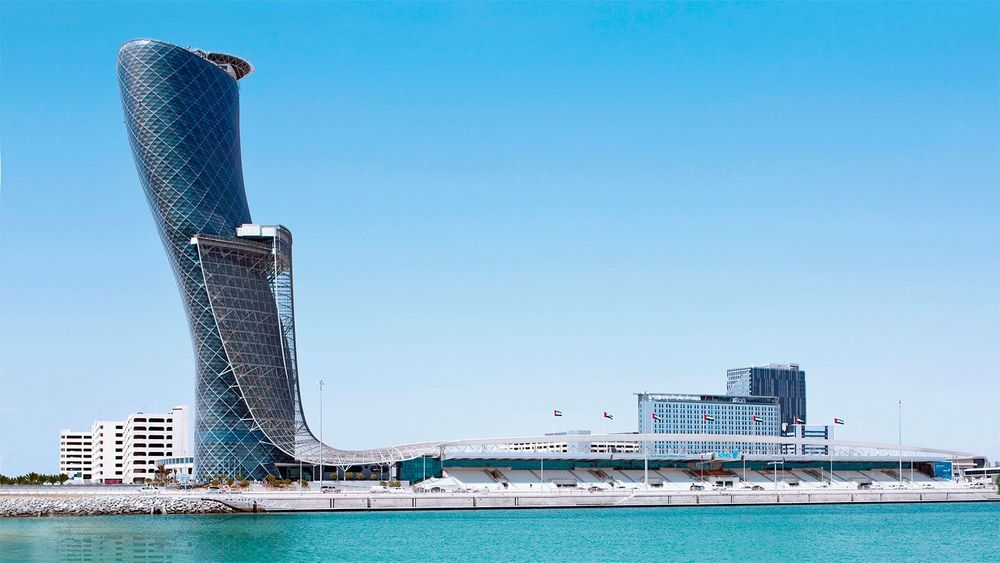
\includegraphics[width=0.9\linewidth]{examples/handbook_coling25/local_guide/images/location.png}
 \end{figure}

\noindent{COLING 2025 is taking place in the Abu Dhabi National Exhibition Centre (ADNEC). ADNEC is a multi-award-winning venue offering organizers of exhibitions, conferences, and events outstanding facilities spread over a total space of 151,000 square meters. ADNEC is just 15 minutes away from the rapidly expanding Abu Dhabi International Airport which serves over 50 airlines and 100 destinations in 46 countries around the globe. It is only 20 minutes from downtown Abu Dhabi and 90 minutes from Dubai International Airport.}\\
\begin{itemize}[noitemsep]
    \item Address: Abu Dhabi National Exhibitions Company, Khaleej Al Arabi Street, P.O. Box 5546, Abu Dhabi, United Arab Emirates
    \item Phone: +971 (0) 2 444 6900
    \item Web: https://adnec.ae/
    \item E-mail: customer.services@adnec.ae
\end{itemize}

\section{Abu Dhabi}

 \begin{figure}[h!]
  \centering
      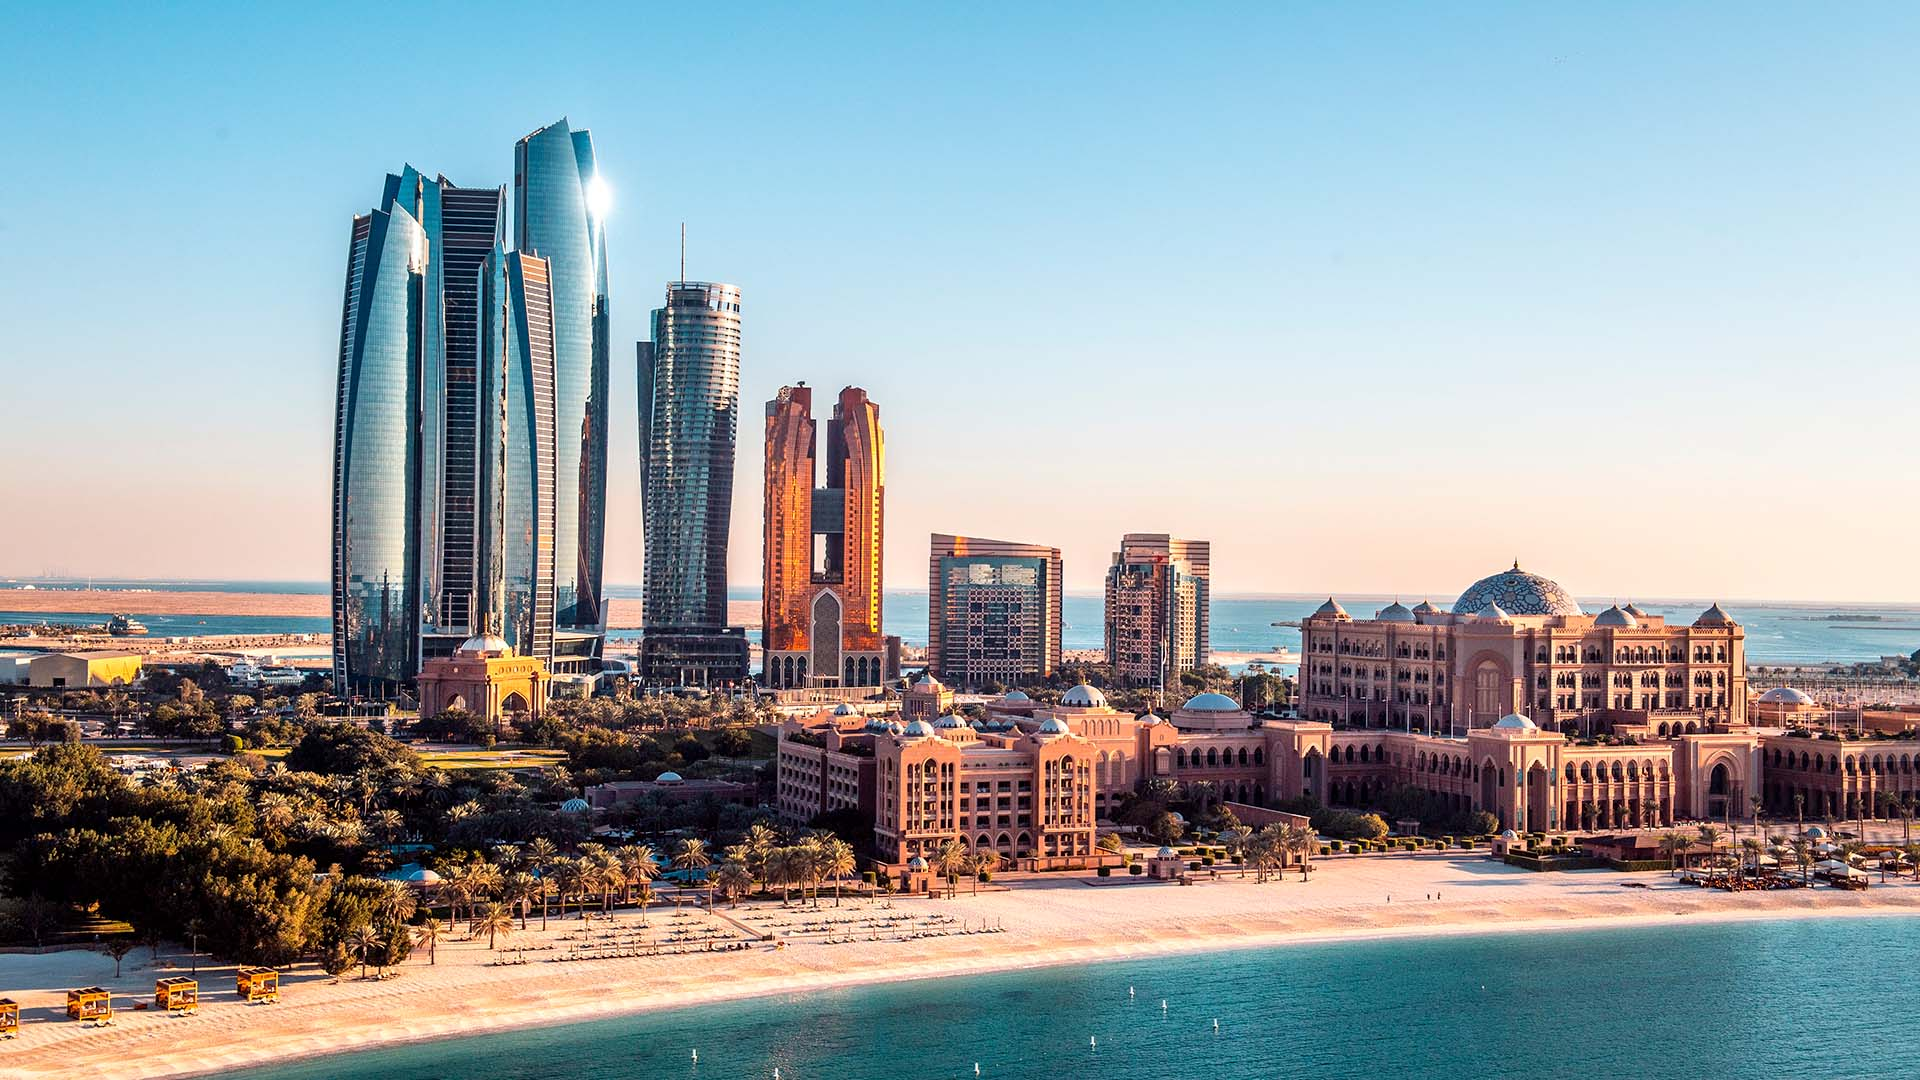
\includegraphics[width=0.9\linewidth]{examples/handbook_coling25/local_guide/images/abu-dhabi.png}
 \end{figure}
 \leavevmode\newline

\noindent{Abu Dhabi, the capital of the United Arab Emirates, is a city of contrasts where traditional meets modern, offering visitors an unforgettable experience.
  Situated on a set of islands in the Arabian Gulf, Abu Dhabi is a cosmopolitan city with a very large international presence (90\% of residents).
 English is the lingua franca.} \\

 \noindent{\large \textbf{Local Transportation in Abu Dhabi}}\\

\begin{itemize}[noitemsep]
    \item ADNEC is just a 20-minute car ride from Abu Dhabi Airport. From Abu Dhabi Corniche, ADNEC is located just 15 minutes away.
    \item \textbf{Taxis} are available throughout Abu Dhabi and they are quite convenient, safe and affordable. You can order a taxi by calling \+971 600 53 53 53 or using the Yango app. A number of taxis are available at Abu Dhabi airport, and from ADNEC at the adjacent Aloft Hotel entrance - look for cars with a "National Taxi" sticker on the side and make sure the driver turns the meter on. UBER is also available in Abu Dhabi but it is generally a bit more expensive than a taxi.
    \item \textbf{Buses} are also available around Abu Dhabi and ADNEC is serviced by bus number 040, seven days a week. More information about bus routes and timings can be found on Google Maps (AppStore, Google Play). A weekly subscription for public transport costs 30 AED and can be purchased at Abu Dhabi Airport, vending machines in the city, and Lulu Supermarkets.
\end{itemize}

\noindent{\large \textbf{Childcare}}\\
\noindent{Please check with the specific hotel where you plan to stay for childcare support.}\\ 

\noindent{\large \textbf{Dining Options}}\\
\noindent{There are a variety of dining selections located near ADNEC. A short walk or drive away, chances are you will find something to satisfy your tastebuds. Use a search engine to find a restaurant near you. There are also a number of cafes and two supermarkets (Zoom and Lulu Express) within a 5 minute walk from ADNEC. Below are recommendations made by a local chair:}\\
\begin{itemize}[noitemsep]
    \item \textbf{Saudi Kitchen} \url{https://maps.app.goo.gl/JXDFdY5UxesJ6Wcu8}
    \begin{itemize}[noitemsep]
        \item Attractive atmosphere (floor seating)
        \item Excellent mandi
        \item Suitable for large groups (10+)
        \item Very affordable
        \item 8-minute ride from ADNEC
    \end{itemize}
    
    \item \textbf{Mosaic} \url{https://maps.app.goo.gl/gkCfGz8xyDaX4yeS8}
    \begin{itemize}[noitemsep]
        \item Elegant but down to earth
        \item Excellent Lebanese dishes
        \item Suitable for group of 8-10
        \item Affordable
        \item 8-minute ride from ADNEC
    \end{itemize}
    
    \item \textbf{Bait El Khetyar} \url{https://maps.app.goo.gl/x8aehmUH2Bh4rY3m8}
    \begin{itemize}[noitemsep]
        \item Casual dining
        \item Excellent hummus, mutabal, and shawarma
        \item Limited seating (but fast for take-away)
        \item Very affordable
        \item 8-minute drive from the Corniche
    \end{itemize}
    
    \item \textbf{Tasha}
    \begin{itemize}[noitemsep]
        \item Casual dining in a nice atmosphere
        \item Excellent Egyptian dishes (mahshi, koshari, etc.)
        \item Good for groups of 8-10
        \item Affordable
        \item 2-minute ride from the Corniche
    \end{itemize}
\end{itemize}

\clearpage

\section{Abu Dhabi Landmarks}

\noindent{\large \textbf{Emirates Palace}}\\
\noindent{Located in the heart of Abu Dhabi, Emirates Palace is one of the capital’s most well-known landmarks.
It is known for its enchanting Arabesque style, award-winning five-star hospitality, and wonderfully unique and authentic local experiences.}\\

\noindent{\large \textbf{Louvre Abu Dhabi}}\\
\noindent{The iconic Louvre Abu Dhabi is the first universal museum in the Arab World, translating and fostering the spirit of openness between cultures.
 As one of the premier cultural institutions located in the heart of the Saadiyat Cultural District on Saadiyat Island,
  this art-lovers’ dream displays works of historical, cultural, and sociological significance, from ancient times to the contemporary era.}\\
 
\noindent{\large \textbf{Sheikh Zayed Grand Mosque}}\\
\noindent{The impressive and inspiring Sheikh Zayed Grand Mosque is one of the world’s largest mosques and the only one that captures the unique interactions between Islam and other world cultures.
 Sheikh Zayed bin Sultan Al Nahyan, the Founder of the UAE, had a very specific vision for this mosque: to incorporate architectural styles from different Muslim civilizations and celebrate cultural diversity by creating a haven that is truly welcoming and inspirational in its foundation.
 The mosque’s architects were British, Italian, and Emirati, with design ideas borrowed from parts of Turkey, Morocco, Pakistan, and Egypt, among other Islamic countries.}\\

\noindent{\large \textbf{Qasr Al Hosn}}\\
\noindent{Over the centuries, Qasr Al Hosn has been home to the ruling family, acted as the seat of government,
housed the National Consultative Council founded by the late Sheikh Zayed Bin Sultan Al Nahyan,
Founder of the UAE, as well as being a national archive. Today it stands as the nation’s living memorial and a narrator of Abu Dhabi’s history.}\\

\noindent{\large \textbf{The National Aquarium Abu Dhabi}}\\
\noindent{The largest aquarium in the Middle East, The National Aquarium in Al Qana is literally swimming with aquatic wildlife featuring over 46,000 animals from more than 300 unique species.
Spread across 10 nautically-themed zones, from the UAE’s Natural Treasures, sunken sea wrecks, and Atlantic caves, right through to flooded forests, fiery volcanoes, and a frozen ocean,
there are more than 60 attractions that will be sure to delight and excite the whole family.}\\

\noindent{\large \textbf{Yas Island}}\\
\noindent{This family-friendly entertainment hub is just a 30-minute drive from the city and a 15-minute drive from Abu Dhabi International Airport.
Yas Island is home to an F1™ race track, several theme parks, an incredible links golf course, a beautiful beach, stunning hotels,
an impressive mall and much more. It’s the perfect place to bring the kids, from toddler to teen, for a fun-filled holiday by the sea.}\\

\noindent{\large \textbf{Jubail Mangrove Park}}\\
\noindent{Jubail Mangrove Park is home to meandering boardwalks that allow you to wander through the mangroves,
discovering a nature-rich side to Abu Dhabi and spotting an array of wildlife, from turtles to herons, gazelle, and more.
Birdwatchers, nature-lovers, and photographers will be in their element here.}\\

\noindent{\large \textbf{Abu Dhabi’s Corniche}}\\
\noindent{Abu Dhabi’s Corniche stretches over eight kilometers of manicured waterfront that includes children’s play areas,
separate cycle and pedestrian pathways, cafés and restaurants, and a lifeguarded beach.}\\

\noindent{\large \textbf{Abu Dhabi Beaches}}\\
\begin{itemize}[noitemsep]
    % \itemsep-0.5em
    \item \textbf{Soul Beach Saadiyat Island}: Tucked away in Saadiyat Island, Soul Beach is Saadiyat Island’s new captivating beachfront location, part of the Mamsha Al Saadiyat community.
    \item \textbf{Saadiyat Beach}: With pristine white sands stretching out along a generous shore, Saadiyat Beach maintains its reputation as one of the most desirable beach locations in the UAE.
    \item \textbf{Yas Beach}: Set on a majestic stretch of white sand, sun-seekers holidaying at any of Yas Island’s hotels and hotel apartments can enjoy complimentary access to the island’s crystal clear waters and natural mangrove surrounds.
    \item \textbf{Corniche Beach}: This beautiful beach isn’t just home to turquoise water and soft, white sand, it also has a beautiful seaside boardwalk, with well-kept walkways home to manicured gardens and benches overlooking the picturesque Arabian Gulf.
    \item You might notice a location not far from ADNEC called "\textbf{Al Qurm Beach}". While this is not a swimming spot, it is a lovely area for a walk, where many locals gather for BBQs and games.
\end{itemize}


 \leavevmode\newline
\section{Important Information}

\noindent{\large \textbf{Climate}}\\
\noindent{Abu Dhabi has a northern-hemisphere subtropical, arid climate. November to March is the most appealing time of year, and it is also when infrequent winter rains occur.
The temperature range in the winter months is between 56 F (13 C) and 75 F (24 C) with typically bright sunny days which correspond to the best kind of spring weather in the US.}\\

\noindent{\large \textbf{Clothing}}\\
\noindent{Summer clothing may be worn for most of the year, but during the winter evening temperatures may occasionally call for a jacket or light coat. 
While dress codes are fairly liberal, consideration should be given not to offend the sensibilities of others. 
Swimwear should be worn only on beaches or at swimming pools. Visiting shopping malls and other attractions, tourists should wear clothing that is not too tight or revealing. 
Certain attractions such as mosques or religious sites usually have stricter dress codes, requiring both men and women to cover up bare shoulders, arms and legs, and women to wear headscarves.}\\

\noindent{\large \textbf{Communications}}\\
\noindent{The international dialing code for incoming calls to landlines in the UAE is +971 and 02 for Abu Dhabi. 
Calls to and from landlines within Abu Dhabi are free. Direct dialing is possible to over 170 countries. 
UAE has two mobile networks, Du and Etisalat:}
\begin{itemize}[noitemsep]
    % \itemsep-0.5em
    \item Both offer temporary SIM cards for tourists and business travelers, including data and calls, and these can be purchased at outlets across the UAE, including at the airport and malls.
    \item Roaming services are also available for most visitors if they wish to use their existing number and phone.
\end{itemize}

\noindent{\large \textbf{Currency and Living Cost}}\\
\noindent{The monetary unit is the Dirham (AED), which is divided into 100 fils. The exchange rate is pegged to the US Dollar at the rate \$1 = AED 3.675.\\
The average costs at an average coffee shop or restaurant are as follows:}
\begin{itemize}[noitemsep]
    % \itemsep-0.5em
    \item Cup of coffee: 14-20 AED/\$3.8-5.5 USD
    \item Sandwich lunch: 15-30 AED/\$5-8.2 USD
    \item Evening meal: 70-100 AED/\$19–27.2 USD
\end{itemize}

\noindent{\large \textbf{Electricity}}\\
\noindent{The electricity supply in Abu Dhabi is 220/240 volts at 50 cycles.
Standard British-type 13-amp square three-pin plugs are the norm in most hotels. 
European or US-made appliances may need a plug adapter.}\\

\noindent{\large \textbf{Language}}\\
\noindent{The official language of the UAE is Arabic. However, English is also very widely spoken throughout Abu Dhabi, 
especially in business, hospitality, retail environments, street signs, taxis, restaurant menus, etc.
Urdu and Hindi are also widely spoken.}\\
\noindent{Top eight phrases to learn:}
\begin{itemize}[noitemsep]
    % \itemsep-0.5em
    \item Marhaba - Hello
    \item Ahlan - Welcome
    \item Ma’asalama - Good Bye
    \item Shukran - Thank you
    \item Mabrook - Congratulations
    \item Yalla - Let’s go
    \item Khalas - enough/done
    \item Inshallah - God willing, may be, no, and a host of other context dependent meanings.
\end{itemize}

\noindent{\large \textbf{Security}}\\
\noindent{As one of the most cosmopolitan and multicultural cities in the world, home to over 200 different nationalities, 
 Abu Dhabi is an advocate for peace and stability, and proud to be a connecting hub between East and West.
Abu Dhabi is ranked in the 10 safest cities by Aon Hewitt, with low crime rates, a stable government,
 and a department of Abu Dhabi Police dedicated entirely to visitors.}\\

\noindent{\large \textbf{Taxation}}\\
\noindent{The UAE does not levy income tax on individuals. Value Added Tax is levied on a majority of goods and services.}\\

\noindent{\large \textbf{Time Zone \& Business Hours}}\\
\noindent{Abu Dhabi is GMT+4. Most businesses are open from 8 am to 6 pm, Monday to Friday,
 with Saturday and Sunday being official holidays for all government departments. 
Embassies, consulates, and government offices operate from 7:30 am to 2:30 pm, Monday to Friday.}\\

\noindent{\large \textbf{Tipping}}\\
\noindent{Tipping practices are similar to most other parts of the world. 
Most restaurants include a 10\% service charge, but tipping, in general, is at the customer’s discretion.}\\

\noindent{\large \textbf{Water}}\\
\noindent{The tap water in Abu Dhabi is safe to drink. But locally bottled water is generally served in hotels and restaurants.}\\

\noindent{\large \textbf{Emergency}\\}
\noindent{The emergency phone number for Abu Dhabi Police is 999. 
Whether you need police assistance, an ambulance, or for any other emergency, 999 is the number to call and calls are free. 
When calling 999, please remember to state your name, the nature of the accident, address of the emergency and how serious the situation is. 
Please find a detailed list of other emergency numbers at the bottom of this page.}

\noindent{If you’re involved in a traffic accident, it’s important to contact the police immediately. 
In case of a minor incident, move your car to the roadside, as there are fines for obstructing traffic. 
Remember, you cannot file an insurance claim without a police report.}

\noindent{For other enquiries, Abu Dhabi Police operates a dedicated Tourism Police section which will advise and guide you on a range of matters. 
You can contact them on +971 2 800 2626 and +971 2 512 7777, or visit Emergency Help for Tourists.}

\noindent{In a medical emergency, Abu Dhabi’s Sheikh Khalifa Medical City (+971 2 819 0000) and Mediclinic Al Noor Hospital (800 2000) both have Accident and Emergency units. 
If you’re injured in a traffic accident, you will automatically be taken to Sheikh Khalifa Medical City, as it has the best Accident \& Emergency treatment facilities.}

\noindent{The Abu Dhabi Government portal provides an updated list of 24-hour pharmacies and medical services, including hospitals, clinics, and medical centres. 
If you don’t have internet access you can call the toll-free number 800 555 (+971 2 666 4442).}\\

\section{Dubai}
\begin{figure}[h!]
 \centering
     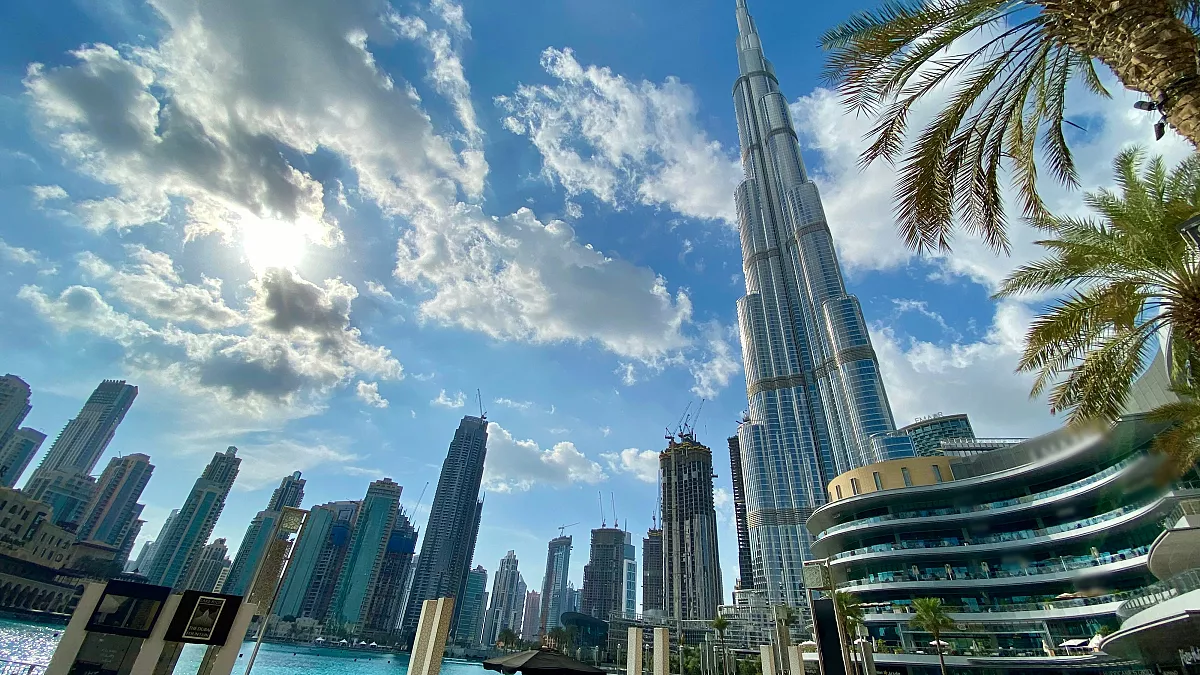
\includegraphics[width=0.9\linewidth]{examples/handbook_coling25/local_guide/images/dubai.png}
\end{figure}
\noindent{Dubai is only 140km (1 hour and 20 minutes by car) away from Abu Dhabi.
 Dubai is a vibrant, urban, and multicultural city with attractive tourist destinations, such as Burj Khalifa – the tallest building in the world.}\\
\clearpage

\section{Sharjah}
\begin{figure}[h!]
 \centering
     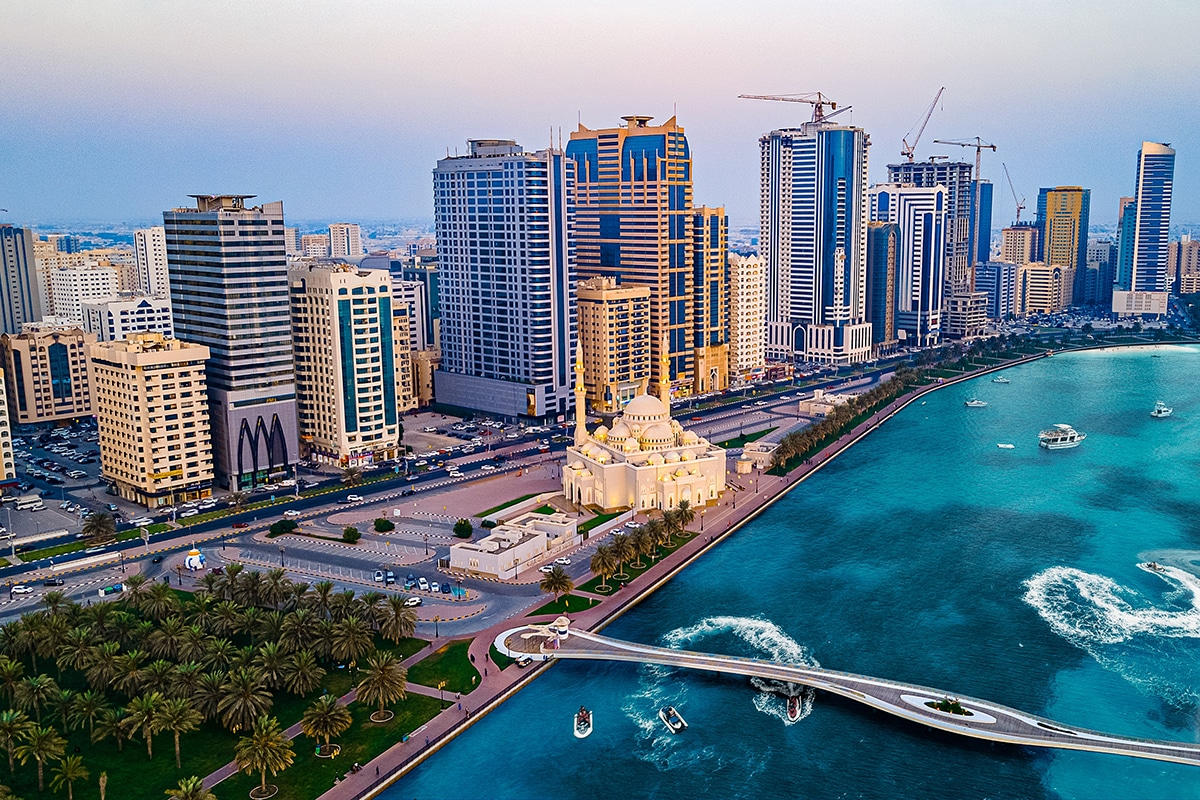
\includegraphics[width=0.9\linewidth]{examples/handbook_coling25/local_guide/images/sharjah.png}
\end{figure}

\noindent{Sharjah is the third largest Emirate, it is only ~165km (1 hour and 50 minutes by car) away from Abu Dhabi.
 It is a major cultural hub in the UAE, there is also a wide variety of activities awaiting. }
